\scanpage{507}
\mspage{556}

But in the more general cases to which we aspire, one must not at \unsure{all} expect $\unsure{\Gamma}_{\rho,\sigma}$ to be so small --- for example that it be commutative.
For example in the ``universal'' case, $\unsure{\mathcal{C}}=\unsure{\mathcal{C}}_{0,3}^{+\wedge}$, we will have
\[
\tag{23}
B_{\rho,\sigma}=\widetilde{M}_{0,3}[0]'=
\operatorname{Ker}\bigl(\widetilde{M}_{0,3}[0]\xrightarrow{\varepsilon_3}\{\pm1\}\bigr)
\]
hence
\[
\tag{24}
\unsure{\Gamma}_{\rho,\sigma}\simeq\widetilde{\Gamma}_{0,3}'
\quad(\supset\Gamma_{\mathbb{Q}}'\ !).
\]

On the other hand, we should be able without inconvenience to postulate the existence of a \inserted{canonical} splitting of the extension $B_{\rho,\sigma}$ of $\Gamma_{\rho,\sigma}$ by $L_0$.
In fact, if we assume, \deleted{$\unsure{\mathcal{C}}$ \unsure{arbitrary}} \deleted{\unsure{that} \illegible{1} \unsure{is}}
\unsure{in} the general case, where nevertheless we assume $\sigma^2=\rho^3=1$, i.e. $\unsure{\mathcal{C}}$ a quotient of $\unsure{\mathcal{C}}_{0,3}^{+\wedge}$, that the quotient $\unsure{\mathcal{C}}$ of $\unsure{\mathcal{C}}_{0,3}^{+\wedge}$ is large enough to map to $\unsure{\mathrm{GP}|\mathrm{CP}}(\widehat{\mathbb{Z}})$, then \deleted{\unsure{that the}} $B_{\rho,\sigma}\simeq\Sigma_{\rho,\sigma}$ maps to $\unsure{\widetilde{B}'_{0,3}|\widetilde{B}'_{0}}$, and the inverse image of $\widetilde{T}_0$ is a subgroup (\unsure{which we could} denote $T_{\rho,\sigma}$)
\[
\tag{25}
T_{\rho,\sigma}\subset B_{\rho,\sigma}\qquad
T_{\rho,\sigma}\xrightarrow{\sim}\unsure{\Gamma}_{\rho,\sigma}
\]
which is a section subgroup, for $B_{\rho,\sigma}\to\unsure{\Gamma}_{\rho,\sigma}$, and also (as a subgroup of $G_{\rho,\sigma}$) for $G_{\rho,\sigma}\to\unsure{\Gamma}_{\rho,\sigma}$, so that we will have
\[
\tag{26}
B_{\rho,\sigma}\simeq T_{\rho,\sigma}.L_0,\quad
G_{\rho,\sigma}\simeq T_{\rho,\sigma}.\unsure{\mathcal{C}}
\qquad\text{($\tfrac12$-direct products)}
\]
\mspage{506}

\scanpage{508}

Now let
\[
\tag{27}
\left\{
\begin{gathered}
\unsure{S_0g}_{\rho,\sigma}^{\deleted{\unsure{\wedge}}}
\deleted{\unsure{\mathcal{C}}}\subset
\unsure{\mathcal{C}}\times\unsure{\mathcal{C}}
\\[-0.3ex]
\Vert\,\mathrm{dfn}
\\
\left\{(\alpha,\beta)\ \middle|\
\underbrace{\alpha\rho(\alpha)^{-1}}_{\unsure{\zeta|\xi}}
=\underbrace{\beta\sigma(\beta)^{-1}}_{\eta}\varepsilon_1^\nu,
\ \text{for }\nu\in\widehat{\mathbb{Z}}\ \text{suitable}\right\}
\\[-0.3ex]
\text{i.e.}\qquad \eta^{-1}\unsure{\zeta|\xi}\in L_1
\end{gathered}
\right.
\]

We have a canonical map
\[
\tag{28}
\left\{\begin{gathered}
\diagram{\begin{tikzcd}[column sep=large,row sep=small]
\unsure{S_0g}_{\rho,\sigma}\deleted{\unsure{\mathcal{C}}}\arrow[r]
  & \Sigma_{\rho,\sigma}\\
(\alpha,\beta)\arrow[r,mapsto]
  & (\unsure{\zeta|\xi},\eta),\quad
\begin{aligned}
\unsure{\zeta|\xi}&=\alpha\rho(\alpha)^{-1}\\
\eta&=\beta\sigma(\beta)^{-1}
\end{aligned}\ ,
\end{tikzcd}}
\end{gathered}\right.
\]
which is a surjection by \deleted{construction}\inserted{definition} of $\Sigma_{\rho,\sigma}$,
and in fact by hypothesis (10) we have \inserted{almost} a
\uline{canonical section}
\[
\deleted{\unsure{(29)}}\qquad
\diagram{\begin{tikzcd}[column sep=large,row sep=small]
\Sigma_{\rho,\sigma}\arrow[r]
  & \unsure{S_0g}_{\rho,\sigma}\deleted{\unsure{\mathcal{C}}}\\
(\unsure{\zeta|\xi},\eta)\arrow[r,mapsto]
  & u_{\unsure{\zeta|\xi},\eta}
\end{tikzcd}}
\]
except that $u_{\unsure{\zeta|\xi},\eta}$ is not in $\unsure{\mathcal{C}}$, but only in $G_{\rho,\sigma}$.
We are going to consider \unsure{the sets|the set} of larger size
\[
\tag{29}
\begin{gathered}
g_{\rho,\sigma}\subset\unsure{G}_{\rho,\sigma}\times\unsure{G}_{\rho,\sigma}
\\[-0.3ex]
\Vert\,\mathrm{dfn}
\\
\left\{(\alpha\beta)\ \middle|\
\underbrace{\alpha\rho(\alpha)^{-1}}_{\unsure{\zeta|\xi}}
=\underbrace{\beta\sigma(\beta)^{-1}}_{\eta}\varepsilon_1^\nu
\quad\text{for }\nu\in\widehat{\mathbb{Z}}\ \text{suitable}\right\}
\\[-0.3ex]
\qquad\deleted{\unsure{\eta^{-1}}}\unsure{\unsure{\zeta|\xi}}
\end{gathered}
\]

\margin{\uline{N.B.} We will also have
$\unsure{\zeta|\xi}=\alpha(\rho)\rho^{-1},\ \eta=\beta(\sigma)\sigma^{-1}$
hence $\unsure{\zeta|\xi},\eta\in\unsure{\mathcal{C}}$ (since
$\unsure{\mathcal{C}}$ \unsure{invariant} in $G_{\rho,\sigma}$)}

so that we will have
\[
\tag{30}
Sg_{\rho,\sigma}=g_{\rho,\sigma}\cap
(\unsure{\mathcal{C}}\times\unsure{\mathcal{C}}).
\]
(assuming (18) to simplify).
\mspage{507}

\scanpage{509}
\mspage{508}
\mspage{557}

\deleted{Thus} We find \unsure{again}
\[
\tag{31}
\left\{\begin{gathered}
\diagram{\begin{tikzcd}[column sep=large,row sep=small]
g_{\rho,\sigma}\arrow[r] & \Sigma_{\rho,\sigma}\\
(\alpha,\beta)\arrow[r,mapsto] & (\unsure{\zeta|\xi},\eta),\quad
\begin{aligned}
\unsure{\zeta|\xi}&=\alpha\rho(\alpha)^{-1}=[\alpha,\rho]=\alpha(\rho)\rho^{\unsure{+1|-1}}\\
\eta&=\beta\sigma(\beta)^{-1}=[\beta,\sigma]=\beta(\sigma)\sigma^{-1}
\end{aligned}
\end{tikzcd}}
\end{gathered}\right.
\]
(by definition of $B_{\rho,\sigma}$ we do indeed find that the $(\unsure{\zeta|\xi},\eta)$ associated with the $(\alpha,\beta)$ are in $\Sigma_{\rho,\sigma}$).
This time hypothesis (10) implies that we have a \uline{canonical section}
\[
\tag{32}
\diagram{\begin{tikzcd}[column sep=large,row sep=small]
\Sigma_{\rho,\sigma}\arrow[r] & g_{\rho,\sigma}\\
(\unsure{\zeta|\xi},\eta)\arrow[r] & (u_{\unsure{\zeta|\xi},\eta},u_{\unsure{\zeta|\xi},\eta})
\end{tikzcd}}
\]
and we find \unsure{the same|the statements} of \S\,48 III).

\uline{Theorem} Let us consider \deleted{the map} subgroups of
$\deleted{\unsure{g}_{\rho,\sigma}}\inserted{G_{\rho,\sigma}}$
\[
\tag{33}
\deleted{\unsure{Z_{\rho,\sigma}}}\quad
\left\{\begin{aligned}
Z_\rho&=\uline{\mathrm{Centr}}_{G_{\rho,\sigma}}(\rho)\\
Z_\sigma&=\uline{\mathrm{Centr}}_{G_{\rho,\sigma}}(\sigma)
\end{aligned}\right.\ ,
\]
\margin{(N.B. in the case $\unsure{\mathcal{C}}=\mathrm{SL}(2,\widehat{\mathbb{Z}})'$ \unsure{etc.}, we will have
\[
Z_\rho=T_\rho,\qquad Z_\sigma=N'_\sigma
\]}
and the product group
\[
B_{\rho,\sigma}\times\unsure{T_\rho}\times\unsure{T_\sigma}
\deleted{\unsure{=S\widetilde{\Gamma}_{\rho,\sigma}}}
\]
then \inserted{we have a} \deleted{\unsure{the}} bijective map
\[
\tag{34}
\diagram{\begin{tikzcd}[column sep=large,row sep=small]
\inserted{B_{\rho,\sigma}\times\unsure{T_\rho|Z_\rho}\times\unsure{T_\sigma|Z_\sigma}}
\deleted{\unsure{S\widetilde{\Gamma}_{\rho,\sigma}}}\arrow[r,"\sim"]
  & g_{\rho,\sigma}\\
(u,a,b)\arrow[r,mapsto] & (ua^{-1},ub^{-1})
\end{tikzcd}}
\]

\margin{by definition of $B_{\rho,\sigma}$ (7) and we see that
$Z_\rho\to B_{\rho,\sigma}$ and $Z_\sigma\to B_{\rho,\sigma}$ are epimorphisms,
hence also their \unsure{composites} $\delta_\rho,\delta_\sigma$ with
$B_{\rho,\sigma}\to\unsure{\Gamma}_{\rho,\sigma}$.
hence the \unsure{maps} (35) are \unsure{epimorphisms.}}

\uline{Corollary}. Let us consider the group homomorphisms
\inserted{$\delta_B:B_{\rho,\sigma}\to\unsure{\Gamma}_{\rho,\sigma},$}
\[
\tag{35}
\left\{
\unsure{\delta_G}:G_{\rho,\sigma}\longrightarrow\unsure{\Gamma}_{\rho,\sigma},
\quad\delta_\rho:Z_\rho\longrightarrow\unsure{\Gamma}_{\rho,\sigma},
\quad\delta_\sigma:Z_\sigma\longrightarrow\unsure{\Gamma}_{\rho,\sigma},
\right.
\]
\inserted{$\delta_B:B_{\rho,\sigma}\to\unsure{\Gamma}_{\rho,\sigma}$}
$\deleted{\delta_B}\unsure{\delta_G}$ is the canonical homomorphism of passage to the quotient
$\unsure{\mathcal{C}}_{\rho,\sigma}=\unsure{\mathcal{C}}$, and
$\delta_\rho,\delta_\sigma\inserted{,\delta_B}$ are the composites of $\unsure{\delta_G}$
with the inclusions $Z_\rho\subset G_{\rho,\sigma},\quad Z_\sigma\hookrightarrow G_{\rho,\sigma},$
\inserted{$B_{\rho,\sigma}\subset G_{\rho,\sigma}$}




\scanpage{510}
\margin{\unsure{denoted} $\unsure{S_0\Gamma^{b}_{\rho,\sigma}}$ \unsure{in} \unsure{the} \S\,48, $\overline{\uline{\mathrm{IX}}}$ ff}

Let
\[
\tag{36}
\deleted{\unsure{S\widetilde{\Gamma}^{0}_{\rho,\sigma}}\unsure{=\widetilde M_{\rho,\sigma}^{0}}\unsure{\subset S_0\Gamma_{\rho,\sigma}}}
\inserted{\unsure{S_0\Gamma^{b_0}_{\rho,\sigma}}}
\subset B_{\rho,\sigma}\times Z_\rho\times Z_\sigma
\]
\[
\begin{gathered}
\Vert\;\mathrm{dfn}\\
\{(u,a,b)\mid\unsure{\delta_G}(u)=\delta_\rho(a)=\delta_\sigma(b)\}.
\end{gathered}
\]
\deleted{i.e. $\unsure{S\Gamma'_{\rho,\sigma}}$} i.e.
\[
\tag{37}
\unsure{S\Gamma'_{\rho,\sigma}}
=B_{\rho,\sigma}\mathbin{\times}_{\unsure{\Gamma}_{\rho,\sigma}}
 Z_\rho\mathbin{\times}_{\unsure{\Gamma}_{\rho,\sigma}}Z_\sigma.
\]
a bijection \deleted{\unsure{here}}
\[
\tag{38}
\diagram{\begin{tikzcd}[column sep=large,row sep=small]
\unsure{S_0\Gamma^{b_0}_{\rho,\sigma}}\arrow[r,"\sim"]
 & S_0g_{\rho,\sigma} \quad\text{(defined in (27))}\\
(u,a,b)\arrow[r,mapsto]
 & \deleted{\unsure{(ua^{-1},ub^{-1})}}\inserted{(\unsure{\zeta|\xi},\eta)},\quad
 \text{with }\unsure{\zeta|\xi}=ua^{-1},\ \eta=ub^{-1}.
\end{tikzcd}}
\]
\margin{N.B. The letter $S$ here is inspired by the usage of \unsure{Mister Ahlfors}
for the ``special Teichmüller groups'', and \unsure{does not at all have}
the same meaning as in $SZ_\rho,SZ_\sigma$, where it indicates that we take
the kernels of $\delta_\rho,\delta_\sigma$ (\unsure{playing the} role of a
``determinant''\ldots)\figure{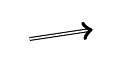
\begin{tikzpicture}\draw[->,double] (0,0)--(0.8,0.12);\end{tikzpicture}}}

\uline{Scholium} By the bijections (34) (38), we transport onto
$\unsure{g}_{\rho,\sigma},\ S_0g_{\rho,\sigma}$ the natural group structures
of $\unsure{\widetilde{\Gamma}_{\rho,\sigma}},\
\unsure{\Gamma^{b_0}_{\rho,\sigma}}$.
Making this group structure explicit we find in particular for $Sg_{\rho,\sigma}$
\[
\tag{\unsure{39|37}}
\left\{\begin{gathered}
(\alpha',\beta')(\alpha,\beta)=\alpha''\beta'',\quad
\text{with }\alpha''=u'(\alpha)\alpha',\quad\beta''=u'(\beta)\beta'.\\
u'=u_{\unsure{\zeta|\xi}',\eta'}:\
\diagram{\begin{tikzcd}[column sep=large]
\unsure{\mathcal{C}}\arrow[r] & \unsure{\mathcal{C}}
\end{tikzcd}},\quad\text{defined by }
\left\{\begin{aligned}
u(\rho)&=\unsure{\zeta|\xi}\rho=\operatorname{int}(\alpha)\rho\\
u(\sigma)&=\eta\sigma=\operatorname{int}(\beta)\sigma
\end{aligned}\right.
\end{gathered}\right.
\]
(with $\unsure{\zeta|\xi}=\alpha\rho(\alpha)^{-1},\ \eta=\beta\sigma(\beta)^{-1}$).

In $\unsure{S_0\Gamma^{b_0}_{\rho,\sigma}}$ we have a subgroup isomorphic to $L_0$, i.e.
\margin{\inserted{
\[
\tag{39}
\diagram{\begin{tikzcd}[column sep=large,row sep=small]
L_0\arrow[r] & \unsure{S\Gamma'_{\rho,\sigma}}\\
\unsure{\ell}\arrow[r,mapsto] & (\ell,1,1)
\end{tikzcd}}
\]
and we have exact sequence
\[
\tag{40}
\diagram{\begin{tikzcd}[column sep=small]
1\arrow[r] & L_0\arrow[r] & \unsure{S\Gamma'_{\rho,\sigma}}\arrow[r]
 & \unsure{\Gamma}_{\rho,\sigma}\arrow[r] & 1
\end{tikzcd}}
\]
}}

\deleted{
$\bullet$ \unsure{Let us now put}
\[
\tag{39}
\begin{gathered}
M_{\rho,\sigma}\subset\operatorname{Aut}(\unsure{\mathcal{C}})\\
\Vert\;\mathrm{dfn}\\
\left\{u\ \middle|\
\begin{array}{l}
\text{\unsure{a)|1°)} }u\ \deleted{\unsure{which}}\ \text{fixes the conjugacy classes of }\rho,\sigma\text{ in }\unsure{\mathcal{C}},\\
\quad\text{i.e. }\exists\alpha_0,\beta_0\in\unsure{\mathcal{C}}\ \deleted{\unsure{\text{such that}}}\ \text{with }\
u(\rho)=\operatorname{int}(\alpha_0)\rho,\quad u(\sigma)=\operatorname{int}(\beta_0)\sigma,\\
\text{\unsure{b)|2°)} }u\ \text{fixes the conjugacy class of }L_0,\\
\quad\text{i.e. }\exists f\in\unsure{\mathcal{C}}\ \text{such that }u(L_0)=\operatorname{int}(f^{-1}).L_0,\\
\quad\text{i.e. }fu\in\operatorname{Norm}_{\operatorname{Aut}(\unsure{\mathcal{C}})}(L_0)
\end{array}\right\}
\end{gathered}
\]
hence by definition of
\[
\tag{41}
\unsure{\mathcal{T}|\Gamma}_{\rho,\sigma}\overset{\mathrm{dfn}}{=}
Z_\rho\mathbin{\times}_{\Gamma_{\rho,\sigma}}Z_\sigma
\]
hence
\[
\tag{42}
\diagram{\begin{tikzcd}[column sep=small]
1\arrow[r] & SZ_\rho\times SZ_\sigma\arrow[r]
 & \unsure{\mathcal{T}|\Gamma}_{\rho,\sigma}\arrow[r,"\unsure{\delta_{\mathcal{T}}}"]
 & \Gamma_{\rho,\sigma}\arrow[r] & 1
\end{tikzcd}}
\]
}
\mspage{509}